\documentclass[10pt]{article}
%\usepackage[latin1]{inputenc} %Eingabezeichensatz
%\usepackage{ngerman}
%\usepackage{amsmath,amssymb,latexsym}
%\usepackage[T1]{fontenc} %europaeische Schriftzeichen
\usepackage{tikz}
%\usepackage{graphics}
%\usepackage{psfig}
%\usepackage{epsfig}


\begin{document}
\pagestyle{empty}

  
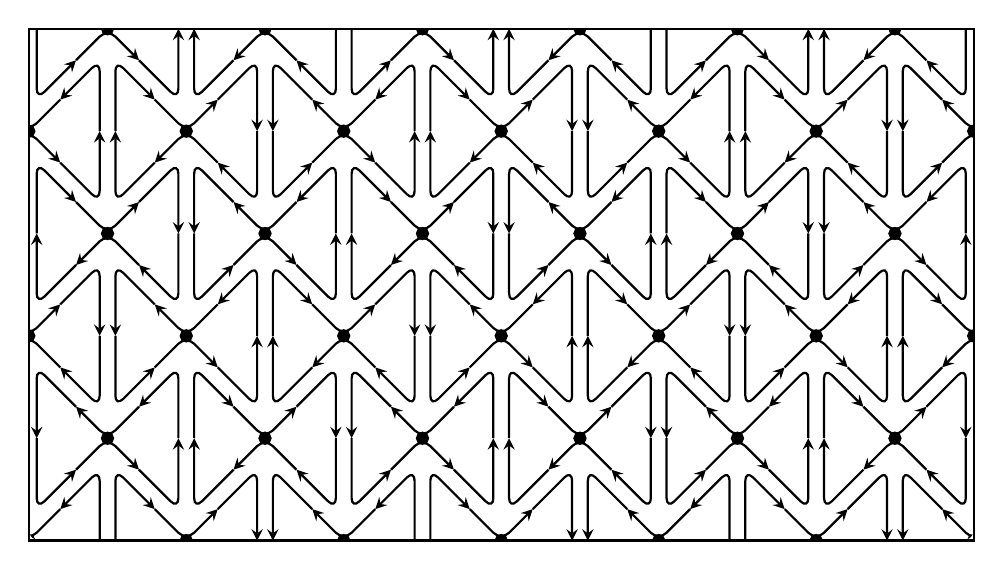
\begin{tikzpicture}[scale=2,rounded corners,rotate=0,>=stealth,thick]
  \foreach \width in {6} 
  \foreach \height in {3.9}
  {
    \draw[rounded corners=0pt] (0,0) rectangle (\width,\height-.65);
    \clip (0,0) rectangle (\width,\height-.65);
    \foreach \y in {0,2.6,...,\height}
    {
      \foreach \x in {0,2,...,\width}
      {
      % simplex
      \draw[->] (\x,\y)+(.2,.2)--+(0,0)--+(-.2,.2); 
      \draw[->] (\x,\y)+(-.2,.2)--+(-.45,.45)--+(-.45,0); 
      \draw[->] (\x,\y)+(-.45,0)--+(-.45,-.45)--+(-.2,-.2); 
      \draw[->] (\x,\y)+(-.2,-.2)--+(0,0)--+(.2,-.2); 
      \draw[->] (\x,\y)+(.2,-.2)--+(.45,-.45)--+(.45,0); 
      \draw[->] (\x,\y)+(.45,0)--+(.45,.45)--+(.2,.2);
      % simplex diagonal above the former
      \draw[->] (\x+.5,\y+.65)+(.2,.2)--+(0,0)--+(-.2,.2); 
      \draw[->] (\x+.5,\y+.65)+(-.2,.2)--+(-.45,.45)--+(-.45,0); 
      \draw[->] (\x+.5,\y+.65)+(-.45,0)--+(-.45,-.45)--+(-.2,-.2); 
      \draw[->] (\x+.5,\y+.65)+(-.2,-.2)--+(0,0)--+(.2,-.2); 
      \draw[->] (\x+.5,\y+.65)+(.2,-.2)--+(.45,-.45)--+(.45,0); 
      \draw[->] (\x+.5,\y+.65)+(.45,0)--+(.45,.45)--+(.2,.2);
      % simplex diagonal under the former
      \draw[->] (\x-.5,\y-.65)+(.2,.2)--+(0,0)--+(-.2,.2); 
      \draw[->] (\x-.5,\y-.65)+(-.2,.2)--+(-.45,.45)--+(-.45,0); 
      \draw[->] (\x-.5,\y-.65)+(-.45,0)--+(-.45,-.45)--+(-.2,-.2); 
      \draw[->] (\x-.5,\y-.65)+(-.2,-.2)--+(0,0)--+(.2,-.2); 
      \draw[->] (\x-.5,\y-.65)+(.2,-.2)--+(.45,-.45)--+(.45,0); 
      \draw[->] (\x-.5,\y-.65)+(.45,0)--+(.45,.45)--+(.2,.2);
      % simplex diagonal under under the former
      \draw[<-] (\x,\y-1.3)+(.2,.2)--+(0,0)--+(-.2,.2); 
      \draw[<-] (\x,\y-1.3)+(-.2,.2)--+(-.45,.45)--+(-.45,0); 
      \draw[<-] (\x,\y-1.3)+(-.45,0)--+(-.45,-.45)--+(-.2,-.2); 
      \draw[<-] (\x,\y-1.3)+(-.2,-.2)--+(0,0)--+(.2,-.2); 
      \draw[<-] (\x,\y-1.3)+(.2,-.2)--+(.45,-.45)--+(.45,0); 
      \draw[<-] (\x,\y-1.3)+(.45,0)--+(.45,.45)--+(.2,.2);
      % intersection point
      \filldraw (\x,\y) circle (1pt);
      \filldraw (\x+.5,\y+.65) circle (1pt);
      \filldraw (\x-.5,\y-.65) circle (1pt);
      \filldraw (\x,\y-1.3) circle (1pt);
      };
      \foreach \x in {1,3,...,\width}
      {
      % simplex
      \draw[<-] (\x,\y)+(.2,.2)--+(0,0)--+(-.2,.2); 
      \draw[<-] (\x,\y)+(-.2,.2)--+(-.45,.45)--+(-.45,0); 
      \draw[<-] (\x,\y)+(-.45,0)--+(-.45,-.45)--+(-.2,-.2); 
      \draw[<-] (\x,\y)+(-.2,-.2)--+(0,0)--+(.2,-.2); 
      \draw[<-] (\x,\y)+(.2,-.2)--+(.45,-.45)--+(.45,0); 
      \draw[<-] (\x,\y)+(.45,0)--+(.45,.45)--+(.2,.2);
      % simplex diagonal above the former
      \draw[<-] (\x+.5,\y+.65)+(.2,.2)--+(0,0)--+(-.2,.2); 
      \draw[<-] (\x+.5,\y+.65)+(-.2,.2)--+(-.45,.45)--+(-.45,0); 
      \draw[<-] (\x+.5,\y+.65)+(-.45,0)--+(-.45,-.45)--+(-.2,-.2); 
      \draw[<-] (\x+.5,\y+.65)+(-.2,-.2)--+(0,0)--+(.2,-.2); 
      \draw[<-] (\x+.5,\y+.65)+(.2,-.2)--+(.45,-.45)--+(.45,0); 
      \draw[<-] (\x+.5,\y+.65)+(.45,0)--+(.45,.45)--+(.2,.2);
      % simplex diagonal under the former
      \draw[<-] (\x-.5,\y-.65)+(.2,.2)--+(0,0)--+(-.2,.2); 
      \draw[<-] (\x-.5,\y-.65)+(-.2,.2)--+(-.45,.45)--+(-.45,0); 
      \draw[<-] (\x-.5,\y-.65)+(-.45,0)--+(-.45,-.45)--+(-.2,-.2); 
      \draw[<-] (\x-.5,\y-.65)+(-.2,-.2)--+(0,0)--+(.2,-.2); 
      \draw[<-] (\x-.5,\y-.65)+(.2,-.2)--+(.45,-.45)--+(.45,0); 
      \draw[<-] (\x-.5,\y-.65)+(.45,0)--+(.45,.45)--+(.2,.2);

      % simplex diagonal under under the former
      \draw[->] (\x,\y-1.3)+(.2,.2)--+(0,0)--+(-.2,.2); 
      \draw[->] (\x,\y-1.3)+(-.2,.2)--+(-.45,.45)--+(-.45,0); 
      \draw[->] (\x,\y-1.3)+(-.45,0)--+(-.45,-.45)--+(-.2,-.2); 
      \draw[->] (\x,\y-1.3)+(-.2,-.2)--+(0,0)--+(.2,-.2); 
      \draw[->] (\x,\y-1.3)+(.2,-.2)--+(.45,-.45)--+(.45,0); 
      \draw[->] (\x,\y-1.3)+(.45,0)--+(.45,.45)--+(.2,.2);


      % intersection point
      \filldraw (\x,\y) circle (1pt);
      \filldraw (\x+.5,\y+.65) circle (1pt);
      \filldraw (\x-.5,\y-.65) circle (1pt);
      \filldraw (\x,\y-1.3) circle (1pt);
      }

    }
  }
\end{tikzpicture}


\end{document}
